\documentclass[lang=en, hanging-titles=true]{skrapport}

\usepackage[backend=biber]{biblatex}
\addbibresource{References.bib}

\usepackage[hidelinks]{hyperref}
\usepackage{graphicx} % allow embedded images
  \setkeys{Gin}{width=\linewidth,totalheight=\textheight,keepaspectratio}
  \graphicspath{{../figs/}} % set of paths to search for images
\usepackage{subcaption}
\usepackage{listings}
\usepackage{listings-rust}
\usepackage{ragged2e}
\usepackage{ctable}
\usepackage{cleveref}
\usepackage{multicol} % multiple column layout facilities

\raggedright
\colortheme{skdoc}
\title{An arm build on Promises}
\author[dskleingeld@gmail.com]{David Kleingeld}

% notes: 
% https://www.rapitasystems.com/blog/what-really-happened-software-mars-pathfinder-spacecraft

\begin{document}

\maketitle
\tableofcontents

\section{Introduction}
Recent years have seen great strides in the field of humanoid robotics. As we get closer to interactions between robots and machines we will need to guarentee safe operations. For this the movement of the robot needs to be strictly controled. Classicly robots are controlled using software build on \textit{real time operating systems} that guarentee strict timing between operations. This at the cost of limitations and complexity. This complexity offers many opportunities for unsafe mistakes. Here I try an alternative; controlling a robot arm without threads, OS or heap while also preventing nearly all memory bugs. This while using easy to reason about software primitives. The arm itself is very simple, constructed out of lego and limited to planar movement. Control is done by a 64kB microcontroller.

In the next section I will introduce the \textsc{Async} software primitive I use instead of threads to do 'concurrent' work. Then in \cref{sec:impl} I will describe my implementation before discussing how this new approach performs in \cref{sec:results}. Finally I will conclude if I succeeded building a simple robotic arm this way and wheather this approach merits further study.

\section{Async}
Before I can describe my implementation I need to introduce \textsc{Async} a syntactic language feature that allows for easy constuction of asynchronous non blocking functions. \textit{Asynchronous} programming lets us write concurrent, not parallel, tasks while looking awfully similar to normal blocking pragramming. It is a good alternative to \textit{event-driven} programming which tends to be verbose and hard to follow. All \textsc{Async} systems are build around special function that do not return a value but rather a \textit{promise} of a \textit{future} value. When we need the value we tell the program not to continue untill the promise is fulfilled. Lets lok at the example of downloading 2 files:

\begin{lstlisting}[language=rust, style=boxed, tabsize=2]
async fn get_two_sites_async() {
	// Create two different "futures" which, when run to 
	// completion, will asynchronously download the webpages.
	let future_one = download_async("https://www.foo.com");
	let future_two = download_async("https://www.bar.com");

	// Run both futures to completion at the same time.
	let futures_joined = join!(future_one, future_two);
	// Run them to completion returning their return values
	let (foo, bar) = futures_joined.await;
	some_function_using(foo,bar);
}
\end{lstlisting}

Notice the \texttt{async} keyword in front of the function definition it means the function will return a promise to complete in the future. The \texttt{join!} statement on line 8 combines the two promises for a future awnser to a single promise for two awnsers. In line 10 we await or 'block' the program until \texttt{futures\_joined} turns into two value. Those can then be used in normal and async functions.

The caller of our \texttt{async} \textit{get\_two\_sites\_async} function will need to be an another async function that can await \textit{get\_two\_sites\_async}, or it can be an executor. An executor allows a normal function to await async functions.

Lets go through our example again explaining how this mechanism could work. The syntax and workings of async differ a lot here we will look at the language \textit{Rust}. In rust these promises for a future value are called futures. Until the program reaches line 10 no work on downloading the example sites is done. This is not a problem as the results, \textit{foo} and \textit{bar}, are not used before line 11. The runtime will start out working on downloading \texttt{www.foo.com}, probably by sending out a dns request. As soon as the dns request has been send we need to wait for the awnser, we need it to know to which ip to connect to download the site. At this point the runtime will instead of waiting start work on downloading bar where it will run into the same problem. If by now we have recieved an awnser on our dns request for \textit{www.foo.com} the runtime will continue its work on downloading foo. If not the runtime might continue on some other future availible to it that can do work at this point.

\section{Implementation}
\label{sec:impl}
Here I will discuss how I used async to get rid of threads and an the need for OS, how I all but excluded the chance of memory bugs and finally I will show the hardware used and why and how my implementation was written heapless. But before we dive into all that how do I actually control the arm. It consists of three motors. These have controlable direction, power and report whenever they have moved. Each motor is controlled using a double pid loop. The inner loop controls velocity using output power. The outer loop controls position using motor target velocity. This is abstracted using object composition: the arm consists of three hinges (objects) each hinge is composed of a motor object. The hinge controls position and the motor object speed.

\subsection{Threadless concurrency}
By combining async with an endless loop we can maintain multiple perhipherals. The key to this is the composability of futures using \textit{join} and a function called \textit{select}. Each of the motors has a \texttt{async} function \textit{maintain} that controls the speed of the motor by regulating its power. It looks like\footnote{I simplified the rust syntax, see the function \texttt{maintain} in \texttt{motor.rs} \href{https://github.com/dskleingeld/robotic-arm/blob/main/src/hinge/motor.rs}{online}} this:
%
\begin{minipage}{\linewidth} % do not break 
\begin{lstlisting}[language=rust, style=boxed, tabsize=2]
async fn maintain(&mut self) {
	loop {
		select! {
			encoder => self.state.update(dist, spd),
			changed => {
				let speed = self.controls_get_speed()
				self.pid.set_target(speed)
			},
			timeout => self.state.update(0,0),
		}
	}
	let power = self.pid.update(self.state.speed)
	self.driver.set(power)
}
\end{lstlisting}
\end{minipage}
%
The \texttt{loop} on line 2 makes the function run forever. On line 3 \texttt{select!} is a special async function with similar syntax to match statement\footnote{switch/case statement in C}. The \textit{arms} of the select, here \texttt{encoder}, \texttt{changed} and \texttt{timeout}, are futures. The select function concurrently awaits its futures. As soon as one of the futures resolves to a value the code after the arrow (=>) of that future will run. No more work will happen on the other futures and the program continues beyond the select function. That means the code above either:
\begin{enumerate}
	\item Updates the state of the motor
	\item Sets the motors target (pid) target position
	\item Update the state of the motor to reflect standing still
\end{enumerate}
Before calculating and setting the new power for the motor in lines 12 and 13.

To control multiple motors simply join on their maintain futures: 
\begin{minipage}{\linewidth} % do not break 
\begin{lstlisting}[language=rust, style=boxed, tabsize=2]
async fn main() {
	let motor_a = ....  // setup boilerplate
	let motor_b = ....
	let motor_c = ....

	let motor_a = motor_a.maintain()  // future
	let motor_b = motor_b.maintain()  // future
	let motor_c = motor_c.maintain()  // future

	join!(motor_a, motor_b, motor_c)
}
\end{lstlisting}
\end{minipage}
%
Since the join function blocks asynchronously until all its arguments resolve and the maintain futures never resolve\footnote{as they never return a value thanks to their endlessly looping body} the join ends up driving the program forever. To add a tasks simply add it to the join statement. For example to test the motors I include a test future that switches the motors speed every few seconds. It loops over normal synchrounus code to tell the motors to change their speed target and an asynchronous sleep function.

Non of the functions used in \textit{motor maintain} may block. They can only 'block' asynchronously using \textit{await}. This requires async building blocks specifically for embedded systems, these are provided by the \textit{Embassy}\cite{embassy} project.

\subsection{Safe and Unsafe}
The implementation is written in Rust: a high performance memory safe language without carbage collection. It is syntactically quite similar to C++ but guarantees, that our program is free from dangeling pointers (the dreaded segfault). It includes the best build system availible making it trivial to lean on the work on others, which I do extensively here. The culture of safetly around the language makes it ideal for a safe robot arm. In practise this means that on any error the program will \textit{panic} allowing\footnote{you will have to write an panic handling function} for controled shutdown of the motors.

To be able to guarentee safety at compile time the languae needs to be very strict, too strict. To be able to interact with hardware we use an unsafe block. It allows us to do things the language deems unsafe such as dereferencing raw pointers, or setting interrupt routines. For my implementation I only had to use unsafe to setup the encoder. As the encoder needs to update its position on external gpio edges it needs to use interrupts. All the other hardware is safely abstracted around by either the embassy project\cite{embassy} or the Hardware Abstraction Layer (\textsc{HAL}). It provides safe\footnote{by having operations that can fail return a Sum type of the error and return value in case of succes. These sum types must be explicitly handled by us, the caller. We can do this by either panicking the program on error or branching to error handling code on error.} standardized access to the hardwares perhipherals such as the adc and gpios.

\subsection{Hardware and Heapless} \label{sec:hw}
The hardware for this project was limited to what I had available and what the embassy project supported. Eventually I picked the \textit{nrf52832} by nordic semicondutors: a low power system on chip featuring a \textit{64MHz Cortex-M4 32 bit Arm CPU} and 64kB or RAM.The motors used are 11 year old \textit{Lego mindstorm NXT} servo motors, see: \cref{fig:motor}. They feature a 360 ticks per turn optical encoder. The motors are driven by two STMicroelectronics \textit{L298P} dual full-bridge drivers. The arm is constructed out of technical lego pieces as seen in \cref{fig:arm}.
%
\begin{figure}
	\centering
	\begin{subfigure}[b]{0.5\linewidth}
		\centering
		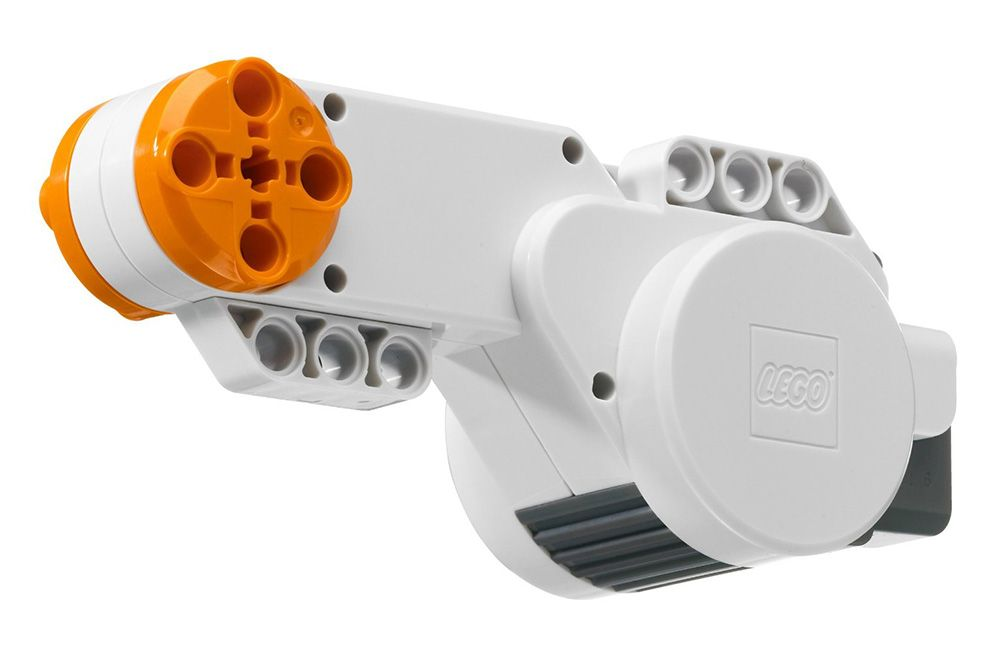
\includegraphics[width=\linewidth]{figs/motor}
		\caption{The mindstorm NXT motor}
		\label{fig:motor}
	\end{subfigure}%
	\begin{subfigure}[b]{0.5\linewidth}
		\centering
		\includegraphics[width=\linewidth]{example-image-b}
		\caption{The lego arm constuction}
		\label{fig:arm}
	\end{subfigure}
\end{figure}
%

The limited amount of ram introduces the risk of heap fragmentation. Imagine a 12kB heap, we first allocate blocks of 4, 5 and then 6 kB before freeing the middle block. Now we have 7kB of free space but can not allocate a block larger then 5Kb, see \cref{fig:heap}. % 
%
\begin{figure}[htbp]
	\centering
	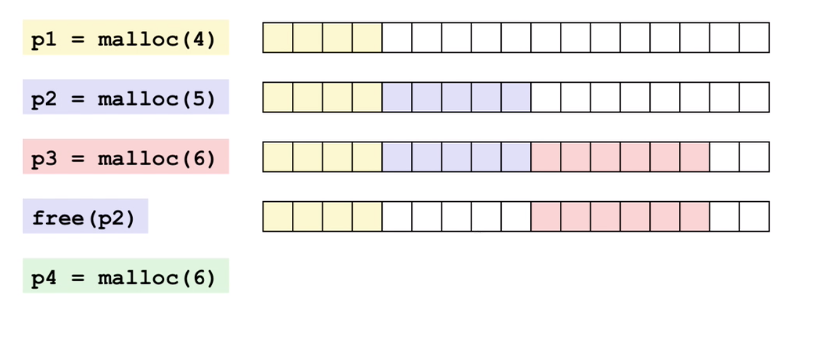
\includegraphics[width=0.9\linewidth]{figs/heapfrag}
	\caption{Heap fragementation illustrated, adapted from \href{https://medium.com/@ankur\_anand/a-visual-guide-to-golang-memory-allocator-from-ground-up-e132258453ed}{Ankur Anand}}
	\label{fig:heap}
\end{figure}
%
With many small and a few large allocations this can happen even with 50\% of the heap still free. Though you can work around this by always allocating the same amount (fixed blocks) I simply chose to only use the stack.

\subsection{Issues}
As async compute on embedded systems is still bleeding edge there where quite a few issues I ran into. 

\begin{enumerate}
	\item To control the motors I needed pwm support, however the HAL did not support this for my chip due to an error in the formal description of the system on chip. I correct this in this \href{https://github.com/nrf-rs/nrf52832-pac/pull/19}{PR} and further upstream in my fork \href{https://github.com/dskleingeld/nrf-hal}{here}
	\item The library providing pid control had an issue preventing compilation on heapless systems I fixed in this \href{https://github.com/yoshuawuyts/pid-lite/pull/1}{PR}.
	\item The encoder needed raw interrupts from the gpio however these where already used by the embassy project to provide an api for async waiting on interrupt changes. I disabled this in my fork \href{https://github.com/dskleingeld/embassy}{here}.
	\item Pins close to eachother could not be used for \textit{PWM}. To discover this I needed to watch the pin output. I could not get an oscilloscope due to an ongoing pandamic. I theirfore build my own, see \href{https://github.com/dskleingeld/rustyscopes}{git}.
\end{enumerate}

\section{Results and Conclusion}
\label{sec:results}
I quantify the performance of the arm by the range of positions it can reach and how fast it moves there. The robot arm is very unstable and takes about 5 seconds to reach a position such as the one in \cref{fig:pos}. This is with one motor. The other motors run freely acting as hinges. To stay stable the \textit{PID} coefficients need to be specifically tuned for each position, rather impractical for such an arm. The \textit{PID} output can only be updated once the encoder gets another tick or when the encoder stays still for 20ms. In practise it runs about every few milliseconds while the arms is moving. As the arm would not be stable with one motor active I did not attempt to control all motors simultaniously.
%
\begin{figure}
	\centering
	\includegraphics[width=0.8\linewidth]{example-image-a}
	\caption{The arm holding position}
	\label{fig:pos}
\end{figure}
%

The cause of the instability is unknown. Here are some possible causes: 
\begin{enumerate}
	\item The lego is too flexible causing vibrations the \textit{PID} control can not deal with. 
	\item The PID loop updates to infrequently and can not deal with the discrete increments in speed/position.
	\item PID coefficients are tuned incorrectly or the implementation is incorrect.
\end{enumerate}
%
I conclude I failed to build a functional robot arm. I do not know why the arm will not move correctly. This does not mean async programming does not show promise. It lead to linear easy to follow and easy to extend code.

\section{Future Work}
Any future work should focus on diagnosing the problem with the \textit{PID} control. A good approach would be to build a traditional interrupt based \textit{PID} control system for the same hardware. If that system proves stable it should be used as reference to find the issue in the async implementation. 

An intresting improvements that can be added is force sensing/limiting. This works by sensing the current draw of the motor, which for servos is related to their output torgue. It was one of the origional goals of this project cancelled due to software and time limitations. For one there is no nonblocking way to get samples from the \textit{ADC} right now. To add force sensing and limiting to the current architecture simply add another \textit{PID} layer controlling trogue using current. Speed should then control torgue.

Furthermore instead of a single Executor to drive all futures with equal priority one could use multiple at different priorities. This at the cost of reinstroducing some of the complexity of event and interrupt driven systems. This it will reduce the time between an encoder update and a change in pid output.

\clearpage
\appendix
\section{Run Instructions}
To try my implementation you will need the hardware listed in \cref{sec:hw}, a STlink V2 programmer and a linux system. First install the rust development environment\footnote{see: https://www.rust-lang.org/learn/get-started}. Then use the setup.sh script in the project root to setup the needed tools for flashing. Now connect the STlink to the nrf52832. To flash and test the program simply run: \texttt{cargo test ---bin test\_hinge}. This will cause the arms lower motor to move between three different positions.

\printbibliography

\end{document}

\pagestyle{scrheadings} % Show chapter titles as headings
\cleardoublepage % Avoids problems with pdfbookmark
